% ============================================================================
%  Inverse Reinforcement Learning: From "How" to "Why"
%  Conference Oral Talk Slides — 17 slides, 15 min
%  Engine: xelatex | Aspect: 16:9 | Venue: NeurIPS
% ============================================================================
\documentclass[aspectratio=169, 11pt]{beamer}

% --- Packages ---
\usepackage{fontspec}
\usepackage{xeCJK}
\usepackage{xcolor}
\usepackage{graphicx}
\usepackage{amsmath, amssymb}
\usepackage{booktabs}
\usepackage{tikz}
\usetikzlibrary{positioning, arrows.meta, calc, shapes.geometric, fit, backgrounds}
\usepackage{tcolorbox}
\tcbuselibrary{skins, breakable}
\usepackage{hyperref}
\usepackage{url}

% --- CJK Fonts ---
\setmainfont{Latin Modern Roman}
\setsansfont{Latin Modern Sans}
\setmonofont{Latin Modern Mono}
\IfFontExistsTF{Microsoft YaHei}{
  \setCJKmainfont{Microsoft YaHei}[BoldFont={Microsoft YaHei Bold}]
  \setCJKsansfont{Microsoft YaHei}[BoldFont={Microsoft YaHei Bold}]
}{
  \IfFontExistsTF{Noto Sans SC}{
    \setCJKmainfont{Noto Sans SC}[BoldFont={Noto Sans SC Bold}]
    \setCJKsansfont{Noto Sans SC}[BoldFont={Noto Sans SC Bold}]
  }{
    \setCJKmainfont{FandolSong-Regular.otf}[
      BoldFont={FandolHei-Regular.otf},
      Path=E:/texlive/2025/texmf-dist/fonts/opentype/public/fandol/]
    \setCJKsansfont{FandolHei-Regular.otf}[
      BoldFont={FandolHei-Bold.otf},
      Path=E:/texlive/2025/texmf-dist/fonts/opentype/public/fandol/]
  }
}

% --- NeurIPS Color Scheme ---
\definecolor{primary}{HTML}{8B5CF6}
\definecolor{accent}{HTML}{2563EB}
\definecolor{accent2}{HTML}{C4B5FD}
\definecolor{good}{HTML}{059669}
\definecolor{warn}{HTML}{F59E0B}
\definecolor{bad}{HTML}{DC2626}
\definecolor{bg}{HTML}{FFFFFF}
\definecolor{text}{HTML}{1E1E1E}
\definecolor{muted}{HTML}{6B7280}
\definecolor{light}{HTML}{F3F4F6}

% --- Beamer Theme ---
\usetheme{default}
\usecolortheme{default}
\setbeamersize{text margin left=0.5cm, text margin right=0.5cm}
\setbeamercolor{frametitle}{fg=primary, bg=bg}
\setbeamercolor{title}{fg=primary, bg=bg}
\setbeamercolor{structure}{fg=accent}
\setbeamercolor{itemize item}{fg=primary}
\setbeamercolor{itemize subitem}{fg=accent}
\setbeamercolor{block title}{fg=white, bg=primary}
\setbeamercolor{block body}{fg=text, bg=light}
\setbeamercolor{block title alerted}{fg=white, bg=bad}
\setbeamercolor{block body alerted}{fg=text, bg=light}
\setbeamercolor{block title example}{fg=white, bg=good}
\setbeamercolor{block body example}{fg=text, bg=light}
\setbeamercolor{normal text}{fg=text, bg=bg}
\setbeamercolor{footline}{fg=muted, bg=bg}
\setbeamertemplate{navigation symbols}{}
\setbeamertemplate{footline}{
  \hfill\insertframenumber\,/\,\inserttotalframenumber\hspace{1.5em}\vspace{0.3em}
}

% --- Custom Commands ---
\newcommand{\hl}[1]{\textcolor{primary}{\textbf{#1}}}
\newcommand{\acc}[1]{\textcolor{accent}{\textbf{#1}}}
\newcommand{\gd}[1]{\textcolor{good}{\textbf{#1}}}
\newcommand{\wn}[1]{\textcolor{warn}{\textbf{#1}}}
\newcommand{\bd}[1]{\textcolor{bad}{\textbf{#1}}}

% Section progress bar
\newcommand{\secbar}[3]{
  \begin{tikzpicture}[baseline=0pt,
      every node/.style={font=\tiny},
      dot/.style={circle, draw=primary!40, fill=primary!10,
        inner sep=0pt, minimum size=4pt},
      doton/.style={circle, draw=primary, fill=primary,
        inner sep=0pt, minimum size=4pt}]
    \foreach \i in {1,...,#2}{
      \pgfmathsetmacro{\filled}{(\i<=#1)?1:0}
      \ifdim \filled pt=1pt
        \node[doton] at (\i*0.18,0) {};
      \else
        \node[dot] at (\i*0.18,0) {};
      \fi
    }
    \node[font=\tiny\color{primary}, anchor=west]
      at (#2*0.18+0.1, 0) {\textbf{#3}};
    \draw[primary!10, line width=0.4pt]
      (0, -0.1) -- (#2*0.18, -0.1);
  \end{tikzpicture}
}

% --- Metadata ---
\title{逆强化学习：从专家行为中读出"为什么"}
\subtitle{Inverse Reinforcement Learning — Theory, Practice \& Frontiers}
\author{MiniMax \and ARIS Research Showcase}
\institute{}
\date{2026}

% --- Custom Title Page ---
\setbeamertemplate{title page}{
  \begin{center}
    \vspace{0.5cm}
    
\begin{tikzpicture}
      \node[circle, draw=primary, line width=2pt,
        minimum size=1.6cm, text=primary] at (0,0) {\Huge$\pi$};
    \end{tikzpicture}
    \\[0.3em]
    {\color{primary}\rule{4cm}{2pt}}\\[0.5cm]
    {\Huge\bfseries\color{primary}\inserttitle}\\[0.3cm]
    {\Large\color{text}\insertsubtitle}\\[0.5cm]
    {\large\insertauthor}\\[0.2em]
    {\color{muted}\insertdate}
  \end{center}
}

\begin{document}

% =========================================================================
%  SLIDE 1: Title
% =========================================================================
\begin{frame}[plain]
  \titlepage
\note{欢迎来到逆强化学习的分享。我是来自 MiniMax 的研究者。
今天用15分钟带大家理解 IRL 的核心思想和发展脉络。}
\end{frame}

% =========================================================================
%  SLIDE 2: Motivation
% =========================================================================
\begin{frame}{Motivation: 奖励工程的痛点}
  \secbar{1}{5}{问题与动机}

  \begin{columns}[T]
    \column{0.52\textwidth}
    \begin{alertblock}{现实困境：奖励函数很难写}
      \begin{itemize}\setlength\itemsep{4pt}
        \item 自动驾驶：撞车 $-100$，变道 $-1$，加速 $+0.1$
        \item 推荐系统：短期点击 vs 长期满意度？
        \item 机器人操控："抓取成功"如何量化？
        \item 对话系统："有帮助"怎么定义？
      \end{itemize}
    \end{alertblock}

    \column{0.48\textwidth}
    \begin{exampleblock}{但行为数据大量存在}
      \begin{itemize}\setlength\itemsep{4pt}
        \item 人类司机每天 \gd{数百万条}轨迹
        \item 老司机 30 年 = 示范黄金库
        \item LLM 阅读 1T+ token 文本
      \end{itemize}
    \end{exampleblock}
    \vspace{0.3cm}
    \begin{center}
      \begin{tcolorbox}[colback=primary!8, colframe=primary,
          arc=4pt, boxrule=0.5pt, width=0.92\textwidth]
        \centering\large\color{primary}\bfseries
        能否 \underline{从示范反推奖励}？
      \end{tcolorbox}
    \end{center}
  \end{columns}

  % Compact outline footer
  \vspace{-0.15cm}
  \begin{center}
    \begin{tikzpicture}[every node/.style={font=\tiny, inner sep=3pt},
        sec/.style={rectangle, rounded corners=3pt, draw=primary!30,
          fill=primary!5, minimum height=0.35cm, align=center},
        arr/.style={-{Stealth[length=1.5mm]}, line width=0.4pt, color=primary!50}]
      \node[sec] (s1) {动机};
      \node[sec, right=0.12cm of s1] (s2) {形式化};
      \node[sec, right=0.12cm of s2, fill=primary!20, draw=primary]
        (s3) {\color{primary}\bfseries 算法演进 $\uparrow$};
      \node[sec, right=0.12cm of s3] (s4) {应用};
      \node[sec, right=0.12cm of s4] (s5) {前沿};
      \draw[arr] (s1)--(s2)(s2)--(s3)(s3)--(s4)(s4)--(s5);
    \end{tikzpicture}
  \end{center}

\note{首先问大家一个问题：你们有没有被奖励函数设计折磨过？
现实世界中奖励很难精确写出来，但人类示范数据却大量存在。
IRL 的核心问题就是：能不能从这些示范中反推出奖励函数？}
\end{frame}

% =========================================================================
%  SLIDE 3: RL vs IRL
% =========================================================================
\begin{frame}{RL vs IRL: 把箭头反过来}
  \secbar{1}{5}{问题与动机}

  \begin{columns}[T]
    \column{0.48\textwidth}
    \centering
    \begin{tikzpicture}[node distance=0.6cm,
        every node/.style={font=\footnotesize},
        box/.style={rectangle, rounded corners, draw, minimum width=1.8cm,
          minimum height=0.65cm, align=center},
        arr/.style={-{Stealth[length=2.5mm]}, line width=1.2pt}]
      \node[box, fill=accent!10, draw=accent] (M) {环境 $M$};
      \node[box, fill=good!10, draw=good, right=of M] (R) {奖励 $r$};
      \node[box, fill=primary!10, draw=primary, right=of R] (pi) {策略 $\pi^*$};
      \node[box, fill=good!10, draw=good, below=1cm of M] (tau) {示范 $\tau_E$};
      \draw[arr, color=accent] (M) -- node[above, font=\scriptsize] {已知} (R);
      \draw[arr, color=primary] (R) -- node[above, font=\scriptsize] {RL} (pi);
      \draw[arr, color=accent, dashed] (pi.south) to[bend right=20]
        node[below, font=\scriptsize] {采样} (tau.east);
      \draw[arr, color=primary, line width=1.8pt]
        (tau.north) to[bend left=30]
        node[right, font=\scriptsize, color=primary] {\bfseries IRL 反推} (R.south west);
    \end{tikzpicture}
    \vspace{0.15cm}
    {\footnotesize\color{primary}\bfseries
      RL: $R \to \pi^*$\quad$\Longleftrightarrow$\quad IRL: $\tau_E \to R$}

    \column{0.52\textwidth}
    \footnotesize
    \begin{tabular}{@{}p{1.3cm}@{\hspace{0.15cm}}p{1.4cm}@{\hspace{0.15cm}}p{1.5cm}@{}}
      \toprule
      \textbf{维度} & \textbf{RL} & \textbf{IRL} \\
      \midrule
      奖励来源 & 人为设计 & \gd{从示范推断} \\
      可解释性 & 弱 & \gd{强} \\
      数据需求 & 在线交互 & \gd{离线可用} \\
      泛化能力 & 受限于塑形 & \gd{可跨环境} \\
      \bottomrule
    \end{tabular}
    \vspace{0.3cm}
    \begin{tcolorbox}[colback=primary!8, colframe=primary,
        arc=3pt, boxsep=2pt, left=4pt, right=4pt, top=3pt, bottom=3pt]
      \centering\footnotesize
      \textbf{\color{primary}IRL 独特价值}\\
      从数据推断 + 强可解释 + 跨环境迁移
    \end{tcolorbox}
  \end{columns}

\note{RL 和 IRL 是同一个硬币的两面。RL 给定奖励求策略，IRL 给定示范反推奖励。
IRL 的独特价值在于：推断出的奖励是可解释的、可迁移到新环境的。}
\end{frame}

% =========================================================================
%  SLIDE 4: MDP + IRL Definition
% =========================================================================
\begin{frame}{数学形式化: MDP 与 IRL 问题定义}
  \secbar{2}{5}{形式化}

  \begin{columns}[T]
    \column{0.5\textwidth}
    \begin{block}{MDP 五元组}
      \centering
      $\langle \mathcal{S}, \mathcal{A}, P, r, \gamma \rangle$
    \end{block}
    \vspace{0.1cm}
    \begin{itemize}\setlength\itemsep{3pt}
      \item $\mathcal{S}$：状态空间
      \item $\mathcal{A}$：动作空间
      \item $P(s'|s,a)$：状态转移
      \item $r(s,a)$：奖励函数
      \item $\gamma \in [0,1)$：折扣因子
    \end{itemize}
    \vspace{0.15cm}
    \begin{block}{RL 目标}
      \centering
      $\pi^* = \arg\max_\pi\;
        \mathbb{E}_{\tau\sim\pi}\bigl[\sum_t \gamma^t r(s_t,a_t)\bigr]$
    \end{block}

    \column{0.5\textwidth}
    \begin{alertblock}{IRL 问题}
      \centering
      已知 $\mathcal{S}, \mathcal{A}, P, \gamma$ 和 $\tau_E$，\\
      \textbf{反求}奖励函数 $r(s,a)$
    \end{alertblock}
    \vspace{0.15cm}
    \begin{center}
      \begin{tcolorbox}[colback=primary!8, colframe=primary,
          arc=3pt, boxsep=2pt, left=4pt, right=4pt]
        \centering\small
        \textbf{\color{primary}关键性质：奖励歧义性}\\
        $r' = r + c$ 不改变最优策略 $\pi^*$
      \end{tcolorbox}
    \end{center}
    \vspace{0.05cm}
    \begin{itemize}\setlength\itemsep{2pt}
      \item $\Rightarrow$ IRL 是 \bd{病态反问题}
      \item $\Rightarrow$ 必须引入 \gd{归纳偏置（先验）}
    \end{itemize}
  \end{columns}

\note{MDP 是 IRL 的数学基础。IRL 给定 MDP 的四元组和专家示范，反求奖励。
但这里有个关键问题：奖励歧义性——给所有状态加一个常数不影响最优策略。
所以 IRL 是一个病态反问题，必须引入归纳偏置。}
\end{frame}

% =========================================================================
%  SLIDE 5: Feature Expectation Matching
% =========================================================================
\begin{frame}{关键洞察: 特征期望匹配}
  \secbar{2}{5}{形式化}

  \begin{columns}
    \column{0.48\textwidth}
    \begin{block}{Ng \& Russell (2000) 核心约束}
      \[
        \mathbb{E}_{\pi_E}[\phi(s,a)]
        \;=\;
        \mathbb{E}_{\pi^*}[\phi(s,a)]
      \]
    \end{block}
    \vspace{0.15cm}
    其中 $\phi: \mathcal{S}\times\mathcal{A} \to \mathbb{R}^k$\\
    是人工设计的 \hl{特征函数}。

    \vspace{0.25cm}
    线性参数化奖励：
    \[ r(s,a) = \theta^\top \phi(s,a) \]

    \column{0.52\textwidth}
    \centering
    \begin{tikzpicture}[scale=0.9,
        every node/.style={font=\footnotesize}]
      \draw[fill=primary!8, draw=primary, rounded corners]
        (0,0) rectangle (5,3.2);
      \node at (2.5, 2.7) {\bfseries\color{primary}求解 $r$ 的思路};
      \node[align=center] at (2.5, 1.6) {
        约束：$\mu_E = \mu_\pi(\theta)$\\[0.3em]
        采用线性规划或\\
        最大边距优化
      };
      \node[color=bad] at (2.5, 0.4) {但解\underline{不唯一}，出现退化};
    \end{tikzpicture}
  \end{columns}

  \vspace{0.25cm}
  \begin{alertblock}{核心问题：如何选择"好"的解？}
    \begin{itemize}\setlength\itemsep{2pt}
      \item \textbf{最大边距}（Abbeel \& Ng 2004）：
        选与最差策略差距最大的 $r$ $\rightarrow$ 不稳定
      \item \hl{\textbf{最大熵}}（Ziebart 2008）：
        选行为最随机（信息量最大）的 $r$ $\rightarrow$
        \gd{唯一解 + 抗噪声！}
    \end{itemize}
  \end{alertblock}

\note{Ng 和 Russell 在 2000 年提出了第一个可操作的 IRL 约束。
但问题在于解不唯一。Ziebart 2008 提出最大熵原则——选择行为最随机的那个解，
给出了唯一解且对噪声鲁棒。这是 IRL 从理论走向实用的关键一步。}
\end{frame}

% =========================================================================
%  SLIDE 6: Algorithm Evolution Timeline
% =========================================================================
\begin{frame}{算法演进：1998 $\to$ 2024}
  \secbar{3}{5}{算法演进}

  \centering
  \begin{tikzpicture}[x=1.4cm,
      every node/.style={font=\small},
      yr/.style={font=\footnotesize\bfseries, color=primary},
      ttl/.style={font=\footnotesize\bfseries},
      desc/.style={font=\scriptsize, color=muted,
        text width=2.6cm, align=center}]

    \shade[left color=primary!5, right color=accent!5]
      (0,-2.0) rectangle (7.2,1.8);
    \draw[line width=2.5pt, color=accent] (0,0) -- (7.2,0);

    \foreach \x/\y in {0/1998, 2.4/2008, 4.8/2016, 7.2/2024} {
      \draw[line width=1.5pt, color=primary] (\x, 0.12) -- (\x, -0.12);
      \node[yr, below=3pt] at (\x, 0) {\y};
      \node[circle, draw=primary, fill=primary,
        inner sep=0pt, minimum size=7pt] at (\x, 0) {};
    }

    \node[ttl, above=8pt] at (0, 0) {Russell};
    \node[desc, above=26pt] at (0, 0) {概念提出\\Ng 2000, Abbeel 04};

    \node[ttl, above=8pt, color=good] at (2.4, 0) {MaxEnt};
    \node[desc, above=26pt] at (2.4, 0) {消除歧义\\Ziebart 2008};

    \node[ttl, above=8pt, color=primary] at (4.8, 0) {GAIL};
    \node[desc, above=26pt] at (4.8, 0) {深度 IRL\\Ho \& Ermon 16};

    \node[ttl, above=8pt, color=primary] at (7.2, 0) {DPO/RLHF};
    \node[desc, above=26pt] at (7.2, 0) {LLM 对齐\\Ouyang 22, Rafailov 23};
  \end{tikzpicture}

  \vspace{0.2cm}
  \begin{tcolorbox}[colback=primary!8, colframe=primary,
      arc=3pt, width=0.8\textwidth, boxsep=2pt]
    \centering\small
    \textbf{\color{primary}核心趋势}: 理论奠基 $\to$
    对抗学习 $\to$ 大模型对齐
  \end{tcolorbox}

\note{IRL 经历了三个重要阶段。1998-2008 是理论奠基期。
Ziebart 2008 的最大熵 IRL 是分水岭。2016 年 Ho 和 Ermon 提出 GAIL。
2022-2024 年 IRL 思想在 LLM 对齐中广泛使用。}
\end{frame}

% =========================================================================
%  SLIDE 7: Classic Pipeline
% =========================================================================
\begin{frame}{经典 Pipeline: 内外双层循环}
  \secbar{3}{5}{算法演进}

  \centering
  \begin{tikzpicture}[
      stp/.style={rectangle, rounded corners, draw=primary,
        fill=primary!5, minimum width=2.0cm, minimum height=0.95cm,
        align=center, font=\footnotesize},
      arrow/.style={-{Stealth[length=2.5mm]}, line width=1pt, color=accent}]

    \node[stp] (s1) {\textbf{STEP 1}\\\\收示范 $\tau_E$};
    \node[stp, right=0.25cm of s1] (s2) {\textbf{STEP 2}\\\\初始化奖励 $r$};
    \node[stp, right=0.25cm of s2] (s3) {\textbf{STEP 3}\\\\RL 求解 $\hat\pi$};
    \node[stp, right=0.25cm of s3] (s4) {\textbf{STEP 4}\\\\匹配 $\mu_E\!\approx\!\mu_{\hat\pi}$};
    \node[stp, right=0.25cm of s4] (s5) {\textbf{STEP 5}\\\\梯度更新 $r$};

    \draw[arrow] (s1) -- (s2);
    \draw[arrow] (s2) -- (s3);
    \draw[arrow] (s3) -- (s4);
    \draw[arrow] (s4) -- (s5);

    \draw[arrow, color=bad, dashed, line width=1.5pt]
      (s5.south) to[out=-90, in=-90, looseness=2.2]
      node[below=4pt, color=bad, font=\scriptsize] {回到 STEP 3}
      (s3.south);
  \end{tikzpicture}

  \vspace{0.3cm}
  \begin{columns}[T]
    \column{0.5\textwidth}
    \footnotesize
    \begin{alertblock}{训练慢的根因}
      \begin{itemize}\setlength\itemsep{2pt}
        \item 外层：推断 $r$（梯度上升）
        \item 内层：RL 求最优 $\hat\pi$
        \item \bd{嵌套} $\Rightarrow$ 高方差 + 极慢
      \end{itemize}
    \end{alertblock}

    \column{0.5\textwidth}
    \footnotesize
    \begin{exampleblock}{GAIL 的解法}
      \begin{itemize}\setlength\itemsep{2pt}
        \item \gd{判别器} = 软奖励信号
        \item 单层对抗，端到端可微
        \item 代价：显式 $r$ 恢复困难
      \end{itemize}
    \end{exampleblock}
  \end{columns}

\note{经典 IRL 是内外双层循环。这种嵌套导致训练非常慢。
GAIL 的创新在于用一个判别器替代显式奖励，把双层优化变成单层对抗。}
\end{frame}

% =========================================================================
%  SLIDE 8: Gridworld Demo
% =========================================================================
\begin{frame}{直观感受: $5\times 5$ 网格世界 IRL}
  \secbar{3}{5}{算法演进}

  \centering
  \begin{tikzpicture}[scale=0.82, transform shape]

    % Left: Expert trajectory
    \node at (-3.5, 0.2) {
      \begin{tikzpicture}[scale=0.48]
        \foreach \r in {0,...,4}
          \foreach \c in {0,...,4} {
            \draw[fill=light] (\c, 4-\r) rectangle (\c+1, 5-\r);
          }
        \draw[->, line width=2pt, color=warn] (0.5,0.5)--(1.5,0.5);
        \draw[->, line width=2pt, color=warn] (1.5,0.5)--(2.5,0.5);
        \draw[->, line width=2pt, color=warn] (2.5,0.5)--(3.5,0.5);
        \draw[->, line width=2pt, color=warn] (3.5,0.5)--(4.5,0.5);
        \draw[->, line width=2pt, color=warn] (4.5,0.5)--(4.5,1.5);
        \draw[->, line width=2pt, color=warn] (4.5,1.5)--(4.5,2.5);
        \draw[->, line width=2pt, color=warn] (4.5,2.5)--(4.5,3.5);
        \draw[->, line width=2pt, color=warn] (4.5,3.5)--(4.5,4.5);
        \node[draw, fill=accent!30, minimum size=0.55cm,
          font=\bfseries\footnotesize] at (0.5,0.5) {S};
        \node[draw, fill=good!70, text=white, minimum size=0.55cm,
          font=\bfseries\footnotesize] at (4.5,4.5) {G};
      \end{tikzpicture}
    };
    \node[font=\bfseries\scriptsize, color=warn] at (-3.3, -2.8)
      {专家示范 (8 步)};

    % Arrow
    \draw[->, line width=2.5pt, color=primary] (-0.5, 0.2) -- (0.5, 0.2);
    \node[font=\Large\color{primary}] at (0, 0.5) {$\mathcal{I}$};

    % Right: Inferred reward heatmap
    \node at (3.5, 0.2) {
      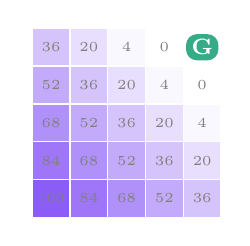
\begin{tikzpicture}[scale=0.48]
        \foreach \row in {0,...,4}
          \foreach \col in {0,...,4} {
            \pgfmathtruncatemacro{\dist}{abs(\col-0) + abs(\row-4)}
            \pgfmathsetmacro{\v}{max(0, 100 - \dist * 16)}
            \fill[primary!\v] (\col, 4-\row) rectangle (\col+1, 5-\row);
            \draw[white, line width=0.5pt]
              (\col, 4-\row) rectangle (\col+1, 5-\row);
            \node[font=\tiny, color=white!50!black]
              at (\col+0.5, 5-\row-0.5)
              {\pgfmathprintnumber[fixed,precision=0]{\v}};
          }
        \node[font=\bfseries\footnotesize, color=white,
          fill=good!80, rounded corners, inner sep=2pt]
          at (4.5, 4.5) {G};
      \end{tikzpicture}
    };
    \node[font=\bfseries\scriptsize, color=primary] at (3.8, -2.8)
      {IRL 推断的奖励热图};
  \end{tikzpicture}

  \vspace{-0.2cm}
  \begin{columns}[T]
    \column{0.55\textwidth}
    \footnotesize
    \textbf{\color{primary}观察：}
    \begin{itemize}\setlength\itemsep{1pt}
      \item \gd{目标格}获得最高奖励值
      \item \gd{奖励山脊}沿最优路径延伸
      \item IRL 对噪声 \gd{鲁棒}
    \end{itemize}

    \column{0.45\textwidth}
    \footnotesize
    \begin{tcolorbox}[colback=primary!8, colframe=primary,
        arc=3pt, boxsep=2pt, left=4pt, right=4pt, top=3pt, bottom=3pt]
      \centering\small
      \textbf{\color{primary}核心结论}\\
      {\scriptsize 从示范反推奖励 = 可解释 + 可迁移 + 抗噪}
    \end{tcolorbox}
  \end{columns}

\note{这是一个简单的 5×5 网格世界演示。左边是专家的最短路径。
右边是 IRL 推断出的奖励热图——越靠近目标奖励越高。}
\end{frame}

% =========================================================================
%  SLIDE 9: MaxEnt IRL
% =========================================================================
\begin{frame}{MaxEnt IRL: 概率化消除歧义}
  \secbar{3}{5}{算法演进}

  \begin{columns}[T]
    \column{0.48\textwidth}
    \begin{block}{核心思想（Ziebart 2008）}
      \centering
      {\large $P(\tau \mid r) \propto
        \exp\!\bigl(\sum_t r(s_t, a_t)\bigr)$}
      \\[0.2em]
      {\footnotesize $\Rightarrow$ 最大似然（拟合） + 最大熵（消歧）}
    \end{block}
    \vspace{0.2cm}
    \begin{alertblock}{梯度方向（简洁！）}
      \centering
      {\Large $\nabla_r \;=\; \mu_E \;-\; \mu_\pi$}
      \\[0.1em]
      {\footnotesize 把 $\mu_\pi$ \gd{拉向} $\mu_E$}
    \end{alertblock}

    \column{0.52\textwidth}
    \centering
    \begin{tikzpicture}[scale=0.85,
        every node/.style={font=\footnotesize},
        box/.style={rectangle, rounded corners, draw,
          minimum width=1.6cm, minimum height=0.6cm, align=center},
        arr/.style={-{Stealth[length=2.5mm]}, line width=1.2pt}]
      \node[box, fill=accent!10] (g) {$\mu_E$};
      \node[box, fill=primary!10, right=1.5cm of g] (p) {$\mu_\pi$};
      \draw[arr, color=primary, line width=1.8pt]
        (p.west) -- node[above, font=\scriptsize] {$\nabla$ 方向} (g.east);
    \end{tikzpicture}

    \vspace{0.3cm}
    \begin{tcolorbox}[colback=good!5, colframe=good,
        width=0.9\textwidth, arc=3pt, boxsep=3pt]
      \centering\small
      \textbf{\color{good}三大优势}\\
      \begin{tabular}{@{}l@{\hspace{0.3cm}}l@{}}
        \gd{✓} 唯一解 & \gd{✓} 凸优化问题\\
        \gd{✓} 抗噪声 & \gd{✓} 充分特征下收敛\\
        \gd{✓} 概率输出 & \gd{✓} 可衡量不确定性
      \end{tabular}
    \end{tcolorbox}
  \end{columns}

\note{MaxEnt IRL 的核心思想很优雅：给每条轨迹赋予概率，奖励越高概率越大。
梯度方向就是专家特征期望减去当前策略期望——非常简洁。}
\end{frame}

% =========================================================================
%  SLIDE 10: GAIL
% =========================================================================
\begin{frame}{GAIL: 用对抗跳过显式奖励}
  \secbar{3}{5}{算法演进}

  \begin{columns}[T]
    \column{0.5\textwidth}
    \begin{block}{核心公式（Ho \& Ermon 2016）}
      \[
        \min_\pi \max_D\;
        \underbrace{\mathbb{E}_{\tau_E}[\log D(\tau)]}_{\text{真专家}}
        \;+\;
        \underbrace{\mathbb{E}_{\tau_\pi}[\log(1-D(\tau))]}_{\text{假策略}}
      \]
    \end{block}
    \begin{itemize}\setlength\itemsep{2pt}
      \item \hl{$D$（判别器）}代替显式奖励 $r$
      \item 等同于 Jensen-Shannon 散度
      \item 端到端可微 — 无需内层 RL
    \end{itemize}

    \column{0.5\textwidth}
    \centering
    \begin{tikzpicture}[scale=0.85,
        every node/.style={font=\footnotesize},
        box/.style={rectangle, rounded corners, draw,
          minimum width=2.0cm, minimum height=0.75cm, align=center},
        arr/.style={-{Stealth[length=2.5mm]}, line width=1.2pt}]

      \node[box, fill=primary!10, draw=primary] (D) {判别器 $D$};
      \node[box, fill=good!10, draw=good, above left=0.8cm and 0.2cm of D]
        (E) {专家 $\tau_E$};
      \node[box, fill=warn!10, draw=warn, below left=0.8cm and 0.2cm of D]
        (G) {策略 $\tau_\pi$};

      \draw[arr, color=good] (E.east) to[bend left=10]
        node[above right, font=\tiny] {$D\!\to\!1$} (D.north west);
      \draw[arr, color=warn] (G.east) to[bend right=10]
        node[below right, font=\tiny] {$D\!\to\!0$} (D.south west);
      \draw[arr, color=primary, dashed, line width=1.5pt]
        (D.west) to[bend left=35]
        node[left, font=\tiny, color=primary] {梯度} (G.west);
    \end{tikzpicture}

    \vspace{0.15cm}
    \begin{alertblock}{局限}
      \begin{itemize}\setlength\itemsep{1pt}
        \item 训练不稳定（GAN 通病）
        \item 奖励不可迁移到新环境
        \item 需要大量在线交互
      \end{itemize}
    \end{alertblock}
  \end{columns}

\note{GAIL 是深度 IRL 的里程碑。它用 GAN 的框架：判别器区分专家和策略，
策略试图骗过判别器。训练端到端，不需要内层 RL 循环。}
\end{frame}

% =========================================================================
%  SLIDE 11: AIRL
% =========================================================================
\begin{frame}{AIRL: 可迁移的奖励}
  \secbar{3}{5}{算法演进}

  \begin{columns}[T]
    \column{0.5\textwidth}
    \begin{block}{核心创新（Fu et al. 2017）}
      \[
        D(s,a,s') = \frac{\exp(f(s,a,s'))}
        {\exp(f(s,a,s')) + \pi(a|s)}
      \]
      其中 $f(s,a,s') = g(s,a) + \gamma h(s') - h(s)$\\
      $\Rightarrow$ 分离 \hl{奖励} 与 \wn{动力学}
    \end{block}
    \vspace{0.1cm}
    \begin{exampleblock}{可迁移性}
      \begin{itemize}\setlength\itemsep{2pt}
        \item 奖励 $g(s,a)$：\gd{环境无关} ✓
        \item 动力学 $h(s)$：环境相关
        \item 迁移 = 只换 $h$，保留 $g$
      \end{itemize}
    \end{exampleblock}

    \column{0.5\textwidth}
    \centering
    \begin{tikzpicture}[scale=0.85,
        every node/.style={font=\footnotesize},
        box/.style={rectangle, rounded corners, draw,
          minimum width=2.2cm, minimum height=0.65cm, align=center},
        arr/.style={-{Stealth[length=2.5mm]}, line width=1.2pt}]

      \node[box, fill=good!10, draw=good] (g) {奖励 $g(s,a)$\\\tiny 可迁移};
      \node[box, fill=muted!15, draw=muted, right=0.6cm of g] (h)
        {动力学 $h(s)$\\\tiny 环境相关};

      \node[box, fill=primary!10, draw=primary, below=0.9cm of g]
        (envA) {环境 A};
      \node[box, fill=accent!15, draw=accent, below=0.9cm of h]
        (envB) {环境 B};

      \draw[arr, color=good, line width=1.5pt] (g.south) -- (envA.north);
      \draw[arr, color=good, line width=1.5pt, dashed]
        (g.south east) to[bend right=15] (envB.north west);
      \draw[arr, color=muted] (h.south) -- (envB.north east);
    \end{tikzpicture}

    \vspace{0.1cm}
    \begin{tcolorbox}[colback=primary!8, colframe=primary,
        arc=3pt, boxsep=2pt, width=0.9\textwidth]
      \centering\small
      \textbf{\color{primary}对抗 + 可分离 = \gd{跨环境泛化}}
    \end{tcolorbox}
  \end{columns}

\note{AIRL 解决了 GAIL 的核心问题：奖励不可迁移。它把奖励和动力学分离，
g 是真正的奖励函数可以跨环境使用，h 捕捉环境特有的动力学。}
\end{frame}

% =========================================================================
%  SLIDE 12: RLHF → DPO
% =========================================================================
\begin{frame}{IRL 的当代化身: RLHF $\to$ DPO}
  \secbar{4}{5}{应用}

  \begin{columns}[T]
    \column{0.48\textwidth}
    \centering
    \begin{tikzpicture}[scale=0.78,
        every node/.style={font=\footnotesize},
        box/.style={rectangle, rounded corners, draw=primary,
          fill=primary!5, minimum width=2.2cm, minimum height=0.65cm,
          align=center},
        arr/.style={-{Stealth[length=2.5mm]}, line width=1pt, color=accent}]

      \node[box] (SFT) {SFT\\\tiny 监督微调};
      \node[box, below=0.35cm of SFT] (RM) {奖励建模 RM};
      \node[box, below=0.35cm of RM] (PPO) {PPO 对齐};
      \node[box, below=0.35cm of PPO, fill=good!10, draw=good]
        (DPO) {\color{good}DPO\\\tiny \color{good}跳过 RM + RL};

      \draw[arr] (SFT) -- (RM);
      \draw[arr] (RM) -- (PPO);
      \draw[arr, color=good, line width=1.5pt]
        ($(SFT.south east)+(0.25,0)$) to[bend right=20]
        node[right, font=\tiny, color=good] {捷径} (DPO.east);
    \end{tikzpicture}

    \column{0.52\textwidth}
    \begin{block}{IRL 视角看 RLHF}
      \[
        \text{偏好数据} \;\xrightarrow{\text{IRL}}\;
        \text{隐式奖励} \;\xrightarrow{\text{RL}}\;
        \text{对齐策略}
      \]
    \end{block}
    \vspace{0.1cm}
    \begin{exampleblock}{关键里程碑}
      \begin{itemize}\setlength\itemsep{3pt}
        \item InstructGPT（Ouyang 2022）\\
          RLHF 让 GPT-3 遵循指令
        \item DPO（Rafailov 2023）\\
          \gd{直接优化偏好，跳过 RL}
      \end{itemize}
    \end{exampleblock}
    \vspace{0.1cm}
    \begin{tcolorbox}[colback=primary!8, colframe=primary,
        arc=3pt, boxsep=2pt, width=0.9\textwidth]
      \centering\small
      \textbf{\color{primary}DPO $\Leftrightarrow$ 隐式 IRL}
    \end{tcolorbox}
  \end{columns}

\note{IRL 的最重要当代应用是 LLM 对齐。RLHF 的奖励建模本质上就是 IRL。
DPO 更进一步——直接优化偏好而跳过显式 RL，数学上等价于隐式 IRL。}
\end{frame}

% =========================================================================
%  SLIDE 13: Application Landscape
% =========================================================================
\begin{frame}{应用图谱: IRL 的落地场景}
  \secbar{4}{5}{应用}

  \centering
  \begin{tikzpicture}[scale=0.82,
      every node/.style={font=\small},
      app/.style={rectangle, rounded corners=6pt, draw=primary,
        fill=primary!8, minimum width=3.2cm, minimum height=1.6cm,
        align=center, font=\footnotesize\bfseries},
      sub/.style={font=\scriptsize, color=muted}]

    \node[app, fill=primary!12] at (0, 3.2)
      (auto) {自动驾驶\\ {\scriptsize\color{muted}MaxEnt IRL, GAIL\\预测人类行为}};
    \node[app, fill=good!8, draw=good] at (6, 3.2)
      (robot) {机器人操控\\ {\scriptsize\color{muted}模仿学习\\从示范到操作}};

    \node[app, fill=accent!8, draw=accent] at (0, 0)
      (llm) {LLM 对齐\\ {\scriptsize\color{muted}RLHF, DPO\\偏好 → 安全}};
    \node[app, fill=warn!8, draw=warn] at (6, 0)
      (game) {游戏 AI\\ {\scriptsize\color{muted}离线 IRL\\从录像学习}};

    \node[app, fill=accent2!30, draw=accent2] at (3, 1.6)
      (rec) {推荐系统\\ {\scriptsize\color{muted}偏好学习\\长期满意度}};
  \end{tikzpicture}

  \vspace{0.15cm}
  \begin{columns}[T]
    \column{0.5\textwidth}
    \footnotesize
    \begin{itemize}\setlength\itemsep{2pt}
      \item 自动驾驶：理解 \gd{为什么变道}
      \item 机器人：从示范学 \gd{操作意图}
      \item LLM 对齐：\gd{当前最大应用场景}
    \end{itemize}
    \column{0.5\textwidth}
    \footnotesize
    \begin{itemize}\setlength\itemsep{2pt}
      \item 游戏 AI：学 \gd{玩家风格}
      \item 推荐系统：学 \gd{真实偏好}
      \item 对话系统：学 \gd{有用性}
    \end{itemize}
  \end{columns}

\note{IRL 的应用非常广泛。自动驾驶用 IRL 理解驾驶意图，
机器人从示范学习操作策略，最大的应用是 LLM 对齐。}
\end{frame}

% =========================================================================
%  SLIDE 14: Open Problems
% =========================================================================
\begin{frame}{开放问题与研究前沿}
  \secbar{5}{5}{前沿}

  \vspace{-0.3cm}
  \begin{columns}[T]
    \column{0.5\textwidth}
    \begin{tcolorbox}[colback=primary!8, colframe=primary,
        arc=4pt, boxsep=4pt, title=\textbf{\color{primary}离线 + 长 Horizon}]
      \footnotesize
      \begin{itemize}\setlength\itemsep{3pt}
        \item 如何使用 \gd{静态数据集}替代在线交互
        \item 长 horizon 任务的分布偏移
        \item 与 Offline RL 的交叉融合
      \end{itemize}
    \end{tcolorbox}
    \vspace{0.15cm}
    \begin{tcolorbox}[colback=good!8, colframe=good,
        arc=4pt, boxsep=4pt, title=\textbf{\color{good}安全与约束 IRL}]
      \footnotesize
      \begin{itemize}\setlength\itemsep{3pt}
        \item 推断的奖励必须 \gd{尊重安全约束}
        \item 约束 IRL：$r$ 在安全区域
        \item 与 RLHF 安全对齐直接相关
      \end{itemize}
    \end{tcolorbox}

    \column{0.5\textwidth}
    \begin{tcolorbox}[colback=accent!8, colframe=accent,
        arc=4pt, boxsep=4pt, title=\textbf{\color{accent}多智能体 IRL}]
      \footnotesize
      \begin{itemize}\setlength\itemsep{3pt}
        \item 多个专家的 \gd{交互奖励}推断
        \item 博弈论 + IRL 的融合
        \item 多智能体价值对齐
      \end{itemize}
    \end{tcolorbox}
    \vspace{0.15cm}
    \begin{tcolorbox}[colback=warn!8, colframe=warn,
        arc=4pt, boxsep=4pt, title=\textbf{\color{warn}IRL + Foundation Model}]
      \footnotesize
      \begin{itemize}\setlength\itemsep{3pt}
        \item 从海量视频/文本 \gd{自动发现奖励}
        \item 预训练先验 + 少量示范微调
        \item 零样本 IRL 的可能性
      \end{itemize}
    \end{tcolorbox}
  \end{columns}

\note{IRL 的开放问题包括：离线设定下的 IRL、安全 IRL、多智能体 IRL，
以及最近非常热门的方向——IRL 与大模型结合。}
\end{frame}

% =========================================================================
%  SLIDE 15: Takeaway
% =========================================================================
\begin{frame}{一页带走: IRL 的核心信息}

  \centering
  \vspace{0.1cm}
  \begin{tikzpicture}[scale=0.88,
      every node/.style={font=\small},
      msg/.style={align=center, font=\large\bfseries, text=primary}]

    \node[draw=primary, fill=primary!5, rounded corners=10pt,
      minimum width=3.5cm, minimum height=2.2cm] at (0, 0) (p1) {};
    \node at (0, 0.4) {\textbf{\color{primary}核心问题}};
    \node[font=\small] at (0, -0.3)
      {如何从示范\\反推奖励函数？};

    \node[draw=accent, fill=accent!5, rounded corners=10pt,
      minimum width=3.5cm, minimum height=2.2cm] at (5.5, 0) (p2) {};
    \node at (5.5, 0.4) {\textbf{\color{accent}核心方法}};
    \node[font=\small] at (5.5, -0.3)
      {MaxEnt: 最大熵消歧\\GAIL: 对抗替代奖励\\AIRL: 可迁移分离};

    \node[draw=good, fill=good!5, rounded corners=10pt,
      minimum width=3.5cm, minimum height=2.2cm] at (11, 0) (p3) {};
    \node at (11, 0.4) {\textbf{\color{good}当代影响}};
    \node[font=\small] at (11, -0.3)
      {RLHF + DPO\\LLM 对齐的核心};

    \draw[->, line width=1.5pt, color=primary!40] (p1.east) -- (p2.west);
    \draw[->, line width=1.5pt, color=primary!40] (p2.east) -- (p3.west);

    % Bottom banner
    \draw[fill=primary!8, draw=primary, rounded corners=8pt]
      (0, -2.0) rectangle (11, -1.0);
    \node at (5.5, -1.5) {\small\bfseries\color{primary}
      奖励 = 行为的"压缩描述" \quad IRL = 从行为反推意图};
  \end{tikzpicture}

\note{总结一下：IRL 从示范反推奖励，MaxEnt/GAIL/AIRL 是核心方法，
当代最大影响在 LLM 对齐。记住：奖励是行为的压缩描述，IRL 反推这个描述。}
\end{frame}

% =========================================================================
%  SLIDE 16: References
% =========================================================================
\begin{frame}{关键参考文献}
  \vspace{-0.3cm}
  \begin{columns}[T]
    \column{0.5\textwidth}
    \footnotesize
    \begin{enumerate}\setlength\itemsep{6pt}
      \item \textbf{Ng \& Russell} (2000)\\
        {\color{muted} Algorithms for IRL. \textit{ICML}.}
      \item \textbf{Abbeel \& Ng} (2004)\\
        {\color{muted} Apprenticeship learning via IRL. \textit{ICML}.}
      \item \textbf{Ziebart et al.} (2008)\\
        {\color{muted} Maximum entropy IRL. \textit{AAAI}.}
      \item \textbf{Ho \& Ermon} (2016)\\
        {\color{muted} Generative adversarial imitation learning. \textit{NeurIPS}.}
    \end{enumerate}

    \column{0.5\textwidth}
    \footnotesize
    \begin{enumerate}\setlength\itemsep{6pt}
      \setcounter{enumi}{4}
      \item \textbf{Fu et al.} (2017)\\
        {\color{muted} Learning robust rewards with adversarial IRL. \textit{ICLR}.}
      \item \textbf{Christiano et al.} (2017)\\
        {\color{muted} Deep RL from human preferences. \textit{NeurIPS}.}
      \item \textbf{Ouyang et al.} (2022)\\
        {\color{muted} Training language models to follow instructions. \textit{NeurIPS}.}
      \item \textbf{Rafailov et al.} (2023)\\
        {\color{muted} Direct preference optimization. \textit{NeurIPS}.}
    \end{enumerate}
  \end{columns}

  \vspace{0.3cm}
  \begin{center}
    \begin{tcolorbox}[colback=light, colframe=primary!30,
        arc=4pt, boxsep=4pt, width=0.9\textwidth]
      \centering\small
      \textbf{推荐综述}: Arora \& Doshi (2021)\quad
      A survey of IRL. \textit{Artificial Intelligence}.
    \end{tcolorbox}
  \end{center}

\note{这是 IRL 领域最关键的 8 篇论文。如果想深入学习，Arora 和 Doshi 的
综述是一个很好的起点。}
\end{frame}

% =========================================================================
%  SLIDE 17: Thank You
% =========================================================================
\begin{frame}{Thank You}
  \centering
  \vspace{0.8cm}

  {\Huge\bfseries\color{primary}Questions?}

  \vspace{0.8cm}

  
\begin{tikzpicture}[scale=0.55]
    % Simplified QR placeholder
    \draw[fill=text] (0,0) rectangle (5,5);
    \foreach \x in {0,...,4}
      \foreach \y in {0,...,4} {
        \pgfmathsetmacro{\on}{rand > 0.3 ? 1 : 0}
        \ifdim \on pt=1pt
          \fill[white] (\x+0.5, \y+0.5) circle (0.15);
        \fi
      }
    \draw[fill=white, text!80!white] (1.5,1.5) rectangle (3.5,3.5);
    \node[font=\large\bfseries, color=text] at (2.5, 2.5) {IRL};
  \end{tikzpicture}

  \vspace{0.4cm}
  {\color{muted}\small\url{https://github.com/example/irl}}
  \\[0.3em]
  {\color{muted}\footnotesize MiniMax · ARIS Research Showcase · 2026}

\note{谢谢大家。论文和代码可通过屏幕上的链接获取。欢迎大家提问交流。}
\end{frame}

\end{document}
